\documentclass[12pt,a4paper]{report}
\usepackage[margin=1in]{geometry}
\usepackage{amsmath,amssymb,amsthm,mathpazo,graphicx,booktabs,hyperref,xcolor,setspace,caption,algorithm,algpseudocode,titlesec,array}
\usepackage[T1]{fontenc}
\graphicspath{{../results/figures/}}
\hypersetup{colorlinks=true,linkcolor=black,citecolor=black,urlcolor=blue!50!black}
\newtheorem{proposition}{Proposition}[chapter]
\theoremstyle{definition}\newtheorem{definition}{Definition}[chapter]
\newcommand{\fillin}[1]{\colorbox{yellow!50}{#1}}
\makeatletter\newcommand{\tabinput}[1]{\@@input #1 }\makeatother
\onehalfspacing
\titleformat{\chapter}[hang]{\Large\bfseries}{\thechapter.}{0.6em}{}
\titlespacing*{\chapter}{0pt}{0pt}{14pt}
\begin{document}
\begin{titlepage}\centering
{\large B.Tech.\ Project Report\par}\vspace{1.4cm}
{\LARGE\bfseries Adaptive Change Point Detection\\[4pt] in Financial Time Series:\\[4pt] An Empirical Study on the S\&P 500\par}\vspace{1.6cm}
Submitted by\par\vspace{0.2cm}
{\large\bfseries Gaius K Biju\par}
Roll No.\ 23BT3FP59\par\vspace{1.2cm}
Under the supervision of\par\vspace{0.2cm}
{\large\bfseries Prof.\ Buddhananda Banerjee\par}\vspace{1.6cm}
Department of Mathematics\par
Indian Institute of Technology Kharagpur\par\vspace{0.3cm}
\fillin{November 2026}
\end{titlepage}
\pagenumbering{roman}
\chapter*{Abstract}
A change point is a time at which the behaviour of a series changes. Online detection in financial prices is difficult because a smoothing estimator must trade delay against false alarms and because market behaviour itself is non-stationary. Adaptive methods, which revise their own settings as data arrive, are a natural response. Following Musaev, Grigoriev and Kolosov (2024), this project asks whether adaptation improves on a well tuned fixed setting. We compare fixed and adaptive exponential smoothing, fixed and adaptive window least squares, rolling multivariate regression and two-sided CUSUM, and also a machine learning combination of their signals. Tests use simulated markets with known truth and daily S\&P~500 data, with settings chosen on 2005--2014 and a single test on 2015--2022. Adaptation gave no general advantage. In simulated clean trends its effect was negligible; under heavy-tailed switching volatility, adaptive smoothing gained 0.024 in mean $F_1$ while the adaptive window lost 0.030. On the S\&P~500 test period, fixed smoothing scored $F_1=0.765$ and adaptive smoothing $0.737$, a difference too small to separate on 18 turning points. Regression and CUSUM did not clearly beat random alarms under a reversal-based answer key, and machine learning models ($F_1\le 0.500$) did not beat the simple rule. These results support the paper's view that there is no universal detector, and show that any claimed benefit of adaptivity should be measured against a tuned fixed control.
\tableofcontents
\clearpage\pagenumbering{arabic}

\chapter{Introduction}
Prices change continually, yet not every change matters. A portfolio manager, risk officer or regulator wants to know, as early as possible and using only information already available, whether a market has entered a new phase. This is the problem of \emph{online change point detection}.

Two requirements pull against each other. Reacting quickly to every movement produces false alarms, while waiting for strong evidence produces late decisions. Chapter~\ref{ch:maths} shows that this conflict can be stated exactly for exponential smoothing.

Musaev, Grigoriev and Kolosov~\cite{musaev2024} argue that financial prices are poorly described by the classical picture of stationary noise interrupted by abrupt shifts. They redefine a change point as a trend reversal, stress that the result depends on the chosen thresholds and methods, and conclude that no universal solution exists. They propose adapting the structure and parameters of a detector, and offer illustrative examples on minute-level currency data, while listing systematic study of parameters and application to other data as future work.

\section*{Research question and contribution}
Our question is: \textbf{does adapting a detector's settings online improve detection over a single well tuned fixed setting?} This report contributes:
\begin{enumerate}
\item a side-by-side test in which each adaptive method has a fixed counterpart or a benchmark;
\item a quantitative evaluation with fixed scoring rules, separate tuning and testing, paired significance tests and a random alarm baseline, complementing the paper's illustrative examples;
\item short derivations of the bias-variance trade-off and the boundedness of the adaptive gain;
\item a leakage-controlled machine learning comparison.
\end{enumerate}

\chapter{Background}
\section{The classical setting}
Let $y_1,\dots,y_n$ be observations decomposed additively as
\begin{equation}y_k=x_k+v_k,\label{eq:model}\end{equation}
with $x_k$ a systematic component and $v_k$ noise~\cite{musaev2024}. In the classical setting, $v_k$ is stationary, often i.i.d.\ Gaussian, and a change point is an abrupt shift in its location or scale parameters. Reviews are given by Truong et al.\ (2020) and Aminikhanghahi and Cook (2017). Methods may be classified as offline or online, supervised or unsupervised, and univariate or multivariate~\cite{musaev2024}. This study concerns online detection, with offline segmentation used only as an answer key.
\section{Why financial data are harder}
Financial returns display volatility clustering and heavy tails (Cont, 2001). In~\cite{musaev2024} the systematic part is described as a non-periodic oscillation with many local trends, and the noise as non-stationary. Hence parameters estimated over one interval may not apply in the next, which motivates adaptation.
\section{Adaptation in the source paper}
The paper separates \emph{structural} adaptation (choosing the most correlated regressors in a sliding window) from \emph{parametric} adaptation (choosing the window length, smoothing factor and threshold). It notes that correlation estimates are unstable over short windows. A pure bidirectional filter and a precedent-matching approach are also discussed; these are not implemented here. Three apparent slips in the paper were noted while reading: the $N(0,1)$ variance is written as zero, $H_0$ and $H_1$ in Section~2.1 appear interchanged, and false alarms are called Type~II errors, whereas they are normally Type~I errors. We use the standard conventions.

\chapter{Mathematical Formulation}\label{ch:maths}
Throughout, $y_t$ is the log price and all estimators at time $t$ use only $y_1,\dots,y_t$.
\begin{definition}[Reversal-based change point]
Given a size $\Delta>0$, a time $c$ is a \emph{turning point} if $y_c$ is the running extreme of the current directional leg and the series subsequently moves against that leg by at least $\Delta$ before the extreme is replaced.
\end{definition}
\noindent This follows the paper's minimum-move idea, with similar directional-change treatments by Aloud et al.\ (2012). The definition depends on $\Delta$, so sensitivity to it is tested.

\section{Exponential smoothing and its trade-off}
Fixed smoothing, Equation (4) in~\cite{musaev2024}, is
\begin{equation}\hat x_t=\hat x_{t-1}+\alpha(y_t-\hat x_{t-1}),\qquad 0<\alpha\le 1.\label{eq:ewma}\end{equation}
Iterating gives $\hat x_t=\alpha\sum_{j\ge0}(1-\alpha)^j y_{t-j}$ when the start is far in the past, so weights decline geometrically and sum to one.
\begin{proposition}[Delay versus noise]\label{prop:tradeoff}
(a) If $y_t=a+bt$, the steady-state error is $y_t-\hat x_t=b(1-\alpha)/\alpha$. (b) If $y_t=\mu+\varepsilon_t$ with i.i.d.\ $\varepsilon_t$ of variance $\sigma^2$, then $\operatorname{Var}(\hat x_t)=\sigma^2\,\alpha/(2-\alpha)$.
\end{proposition}
\begin{proof}
(a) Let $e_t=y_t-\hat x_t$. From \eqref{eq:ewma}, $e_t=(1-\alpha)(e_{t-1}+b)$. The fixed point is $e=(1-\alpha)b/\alpha$, and it is attracting because $|1-\alpha|<1$ for $0<\alpha<2$.
(b) By independence, $\operatorname{Var}(\hat x_t)=\alpha^2\sigma^2\sum_{j\ge0}(1-\alpha)^{2j}=\alpha^2\sigma^2/(1-(1-\alpha)^2)=\sigma^2\alpha/(2-\alpha)$.
\end{proof}
\noindent As $\alpha$ falls, noise variance falls while delay rises. No fixed $\alpha$ minimises both; this is the mathematical form of the conflict the paper describes.

\section{The alarm rule}
Methods that produce a trend line $\ell_t$ share one rule. Let $d_t\in\{+1,-1\}$ be the current direction. If $d_{t-1}=+1$, an alarm is raised when $\max_{s}\ell_s-\ell_t\ge\delta$, with the maximum over the current leg; the rule is symmetric when $d_{t-1}=-1$. Because the rule is shared, differences among these methods come from the estimator and tuned settings.

\section{Method 1: fixed smoothing}
Apply the alarm rule to \eqref{eq:ewma}, with settings $(\alpha,\delta)$.

\section{Method 2: adaptive smoothing}
The Trigg--Leach scheme (1967) updates $\alpha$ from past one-step errors $e_t=y_t-\hat x_{t-1}$:
\begin{align}
m_t&=m_{t-1}+\phi(e_t-m_{t-1}),\qquad s_t=s_{t-1}+\phi(|e_t|-s_{t-1}),\\
\alpha_{t+1}&=\alpha_{\min}+(\alpha_{\max}-\alpha_{\min})\frac{|m_t|}{s_t},
\end{align}
with $\phi=0.1$ fixed. Errors that mostly share a sign suggest the line has fallen behind, so $\alpha$ rises; errors that alternate cancel in $m_t$, so $\alpha$ stays low.
\begin{proposition}\label{prop:bound}
With $s_0\ge|m_0|$ and $0<\phi\le1$, we have $|m_t|\le s_t$ for all $t$, and hence $\alpha_{t+1}\in[\alpha_{\min},\alpha_{\max}]$.
\end{proposition}
\begin{proof}
By induction and the triangle inequality, $|m_t|\le(1-\phi)|m_{t-1}|+\phi|e_t|\le(1-\phi)s_{t-1}+\phi|e_t|=s_t$.
\end{proof}

\section{Method 3: adaptive window}
With window length $L_t$, fit by ordinary least squares $y_{t-j}=\beta_0+\beta_1(-j)+u_j$ for $j=0,\dots,L_t-1$, and take $\ell_t=\hat\beta_0$, the fitted value today. Let $\hat\sigma_t$ be the residual standard deviation. Before fitting at time $t$, compute the forecast $f_t=\hat\beta_{0,t-1}+\hat\beta_{1,t-1}$ and set
\begin{equation}
L_t=\begin{cases}L_{\min}&\text{if }|y_t-f_t|>c\,\hat\sigma_{t-1},\\ \min(L_{t-1}+1,L_{\max})&\text{otherwise.}\end{cases}
\end{equation}
Under homoscedastic uncorrelated noise, the OLS end-point variance is $\sigma^2\,2(2L-1)/(L(L+1))$, which is about $4\sigma^2/L$ for large $L$. A linear trend is estimated without bias, so unlike \eqref{eq:ewma} the line has no steady lag on a straight trend, at the cost of more noise for equal effective memory. Setting $L_{\min}=L_{\max}$ gives the \emph{fixed window control}, which was added so that Method~3 has a like-for-like comparison. The idea of shrinking a window after change is shared with methods such as ADWIN (Bifet and Gavald\`a, 2007), although our rule is a simple heuristic.

\section{Method 4: regression on related series}
Let $\mathbf r_t\in\mathbb R^m$ hold related log prices. At each $t$, using days $t-L,\dots,t-1$: (i) choose the $k$ series whose returns correlate most with the target's returns (structural adaptation); (ii) fit $y=\beta_0+\boldsymbol\beta^\top\mathbf r^{(k)}+u$ by OLS (parametric adaptation), as in Equations (11)--(14) of~\cite{musaev2024}; (iii) compute the standardised out-of-sample gap
\begin{equation}z_t=\frac{\hat\beta_0+\hat{\boldsymbol\beta}^\top\mathbf r_t^{(k)}-y_t}{\hat\sigma_u}.\end{equation}
An alarm fires when $|z_t|>d^*$ (Equation (16) of the paper) and re-arms when $|z_t|<d^*/2$. Two points need care. First, this detects a broken relationship, not a reversal. Second, regressing non-stationary levels can be spurious unless the series are cointegrated (Granger and Newbold, 1974); we follow the paper's level form, but do not establish cointegration, so $z_t$ is a heuristic signal and not a formal test statistic.

\section{Method 5: CUSUM}
Let $z_t$ be daily returns standardised by the mean and standard deviation over the preceding 250 days. Page's statistic (1954) uses
\begin{equation}S_t^+=\max(0,S_{t-1}^++z_t-\kappa),\qquad S_t^-=\max(0,S_{t-1}^--z_t-\kappa),\end{equation}
and fires when either exceeds $h$, after which both restart. For a Gaussian mean shift from $0$ to $\mu_1$ with unit variance, the log-likelihood ratio increment is $\mu_1(z_t-\mu_1/2)$. Dividing by $\mu_1$ gives $\kappa=\mu_1/2$, which is the sense in which CUSUM is derived from sequential likelihood ratio testing. It targets a return-mean shift rather than a price-based reversal.

\section{Scoring}
For true times $\{c_i\}$ and alarm times $\{a_j\}$, each $c_i$ claims the first unused alarm in $[c_i,c_i+H]$. Early alarms earn no credit. With $\text{TP}$ matched pairs, precision is $\text{TP}/\#\{a_j\}$, recall is $\text{TP}/\#\{c_i\}$ and $F_1$ is their harmonic mean. We use $H=40$ trading days, and delay is $a_j-c_i$ for matched pairs. The rules were fixed before results were inspected.

\chapter{Experimental Design}
\section{Simulated markets}
Each run has 1500 days, with segments of random length from 120 to 300 days. Log returns are simulated in three cases.
\begin{itemize}
\item \textbf{Case A, clean trends.} Drift alternates in sign with size uniform on $[0.002,0.004]$; noise is $N(0,0.01^2)$. Truth is each drift reversal.
\item \textbf{Case B, wild noise.} As Case A, with scaled Student-$t_4$ noise and a volatility level switching among $0.006$, $0.01$ and $0.02$. Truth is again each drift reversal.
\item \textbf{Case C, relationship breaks.} Target and related series share a market factor without planted reversals. In alternate segments the target gains extra drift of size uniform on $[0.002,0.004]$ with random sign. Truth is each start and end of a break.
\end{itemize}
Each method is tuned per case by maximising mean $F_1$ across 30 runs, then scored on 200 runs with unseen seeds, after a 250-day burn-in.
\section{S\&P 500 data}
We use daily closes of the S\&P~500 and 20 large US companies from the data bundled in the skfolio package~\cite{skfolio}, from 2 January 2004 to 28 December 2022 (4781 days). Sample index values were checked against well-known closes. Data from 2004 serve as burn-in only. Log prices are used, and non-trading days are not filled. Settings are chosen on 2005--2014, then applied once to 2015--2022. The 10\% hindsight rule gives 18 turning points in each period (Figure~\ref{fig:price}).
\begin{figure}[ht]\centering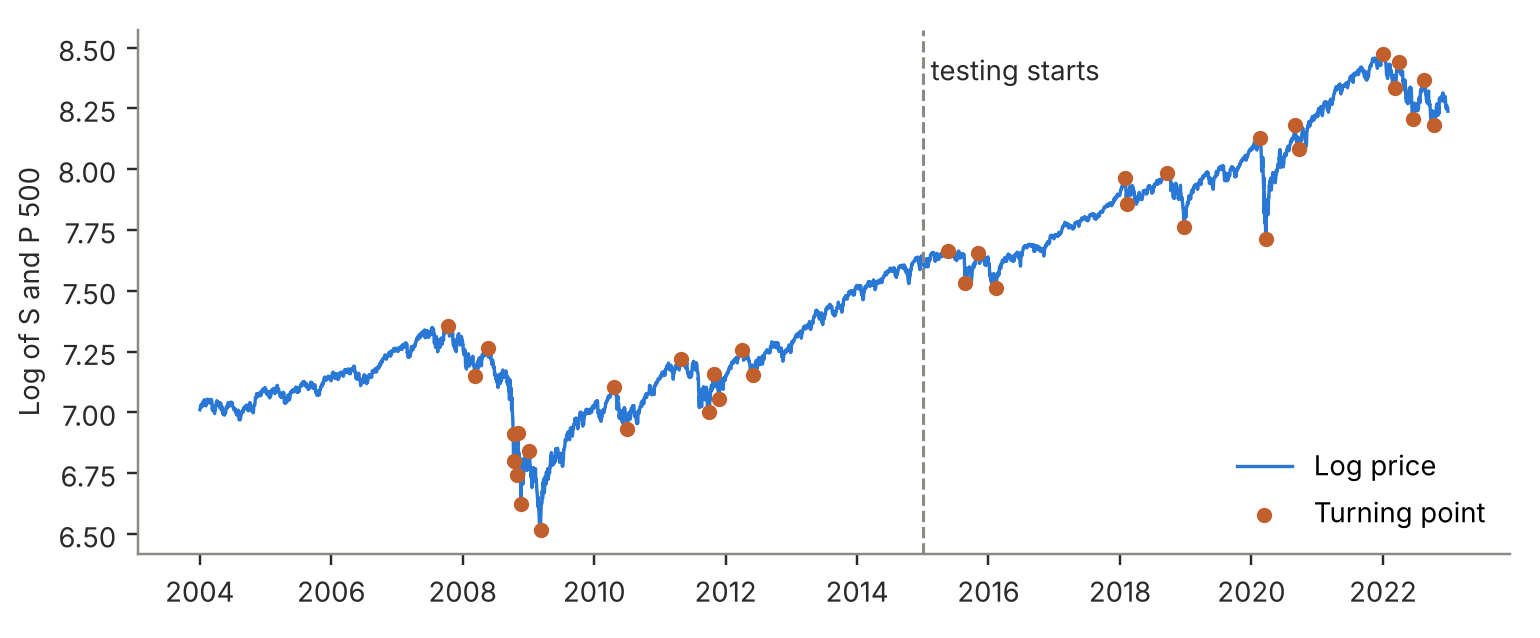
\includegraphics[width=\linewidth]{sp500_turning_points.png}
\caption{S\&P 500 log price with 10\% hindsight turning points.}\label{fig:price}\end{figure}
\section{Statistical checks}
\textbf{Paired tests.} For simulations, per-run $F_1$ differences are assessed with the Wilcoxon signed-rank test (Wilcoxon, 1945), and means have 95\% bootstrap intervals. \textbf{Random alarm test.} For real data, we draw the same number of alarm days uniformly, 2000 times, and compute a one-sided $p$-value. It asks whether alarm timing has skill relative to chance at the same alarm rate. It ignores clustering in market turning points, so it is a rough guide; no correction for multiple comparisons is applied.

\section{Machine learning design}
The target at day $t$ is whether a turning point occurred in the last 20 trading days. Eighteen inputs, all computed from past data, include returns, volatility, distances from highs and lows, smoothing gaps, $\alpha_t$, $L_t$, $z_t$ and CUSUM totals. Models are logistic regression and gradient boosting~\cite{sklearn}. To prevent leakage from the answer key, each training key is computed only from prices before the training cutoff. The alarm level is chosen from expanding-window predictions on 2009--2014. Alarms use an upward crossing and a 20-day wait, and are scored by the rules above.

\chapter{Results}
\section{Simulated markets}
Table~\ref{tab:sim} and Figure~\ref{fig:sim} give the results; paired tests are in Table~\ref{tab:paired}.
\begin{table}[ht]\centering\small
\caption{Test results on 200 unseen simulated runs. Brackets are 95\% bootstrap intervals; FA/1000 is false alarms per 1000 days.}\label{tab:sim}
\begin{tabular}{lccccc}\toprule
Method & Mean $F_1$ & Precision & Recall & Delay & FA/1000\\
\tabinput{tables/simulation.tex}
\bottomrule\end{tabular}\end{table}
\begin{figure}[ht]\centering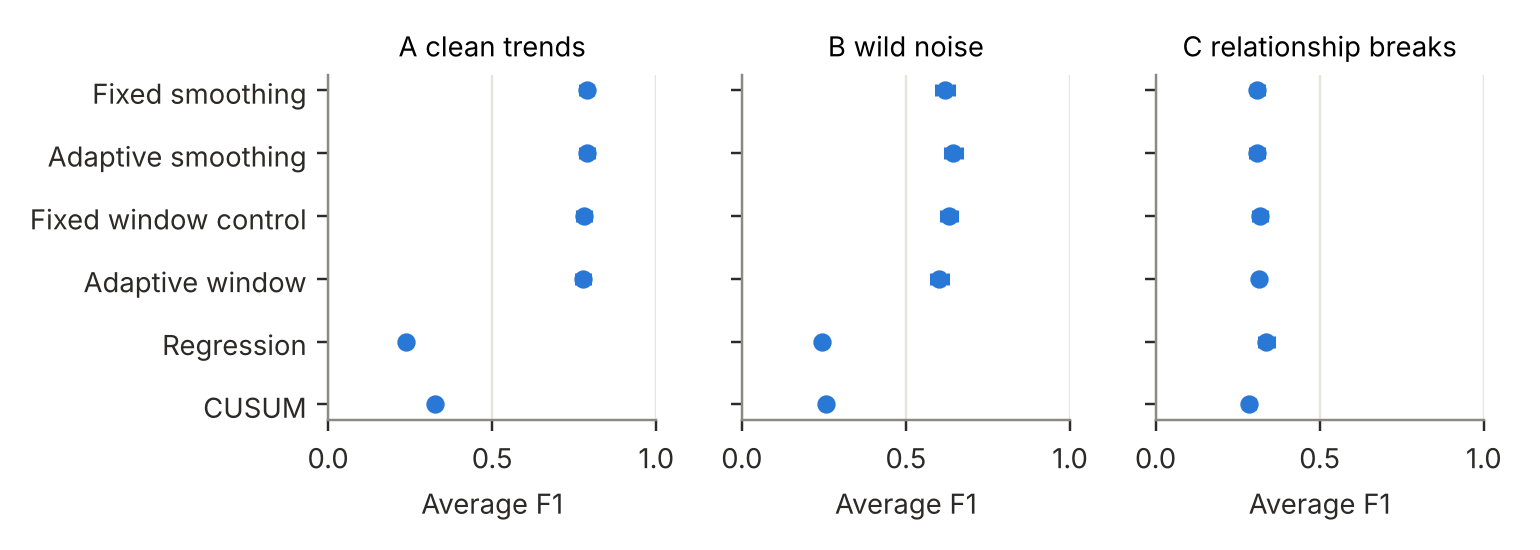
\includegraphics[width=\linewidth]{simulation_f1.png}
\caption{Mean $F_1$ with 95\% intervals on simulated markets.}\label{fig:sim}\end{figure}
\begin{table}[ht]\centering\small
\caption{Paired comparisons of per-run $F_1$ on simulated markets (Wilcoxon signed-rank).}\label{tab:paired}
\begin{tabular}{llcc}\toprule Case & Comparison & Mean difference & $p$\\\midrule
\tabinput{tables/paired.tex}
\bottomrule\end{tabular}\end{table}

\noindent The main findings are:
\begin{itemize}
\item \textbf{Adaptation had no general effect.} In Case A neither adaptive method differed noticeably from its fixed counterpart. In Case B, adaptive smoothing gained 0.024 ($p<0.001$) while the adaptive window lost 0.030 ($p=0.001$). In Case C, neither differed noticeably.
\item \textbf{Method and target must match.} Trend methods far exceeded CUSUM and regression in Cases A and B. Regression was top in Case C at 0.338, and beat CUSUM by 0.051 ($p<0.001$), but its interval overlaps those of the trend methods.
\item \textbf{Case C is hard for all methods.} No method exceeded $F_1=0.34$, so these relationship breaks are not detected well by any method tested.
\end{itemize}

\section{S\&P 500}
Table~\ref{tab:test} shows the single test. Figure~\ref{fig:alarms} shows the timing of alarms.
\begin{table}[ht]\centering\small\setlength{\tabcolsep}{4pt}
\caption{S\&P 500 test period, 2015--2022, with 18 turning points. Random $F_1$ is the mean for random alarms at the same count.}\label{tab:test}
\begin{tabular}{lcccccccc}\toprule
Method & Alarms & Hits & Prec. & Recall & $F_1$ & Delay & Random $F_1$ & $p$\\\midrule
\tabinput{tables/sp500_test.tex}
\bottomrule\end{tabular}\end{table}
\begin{figure}[ht]\centering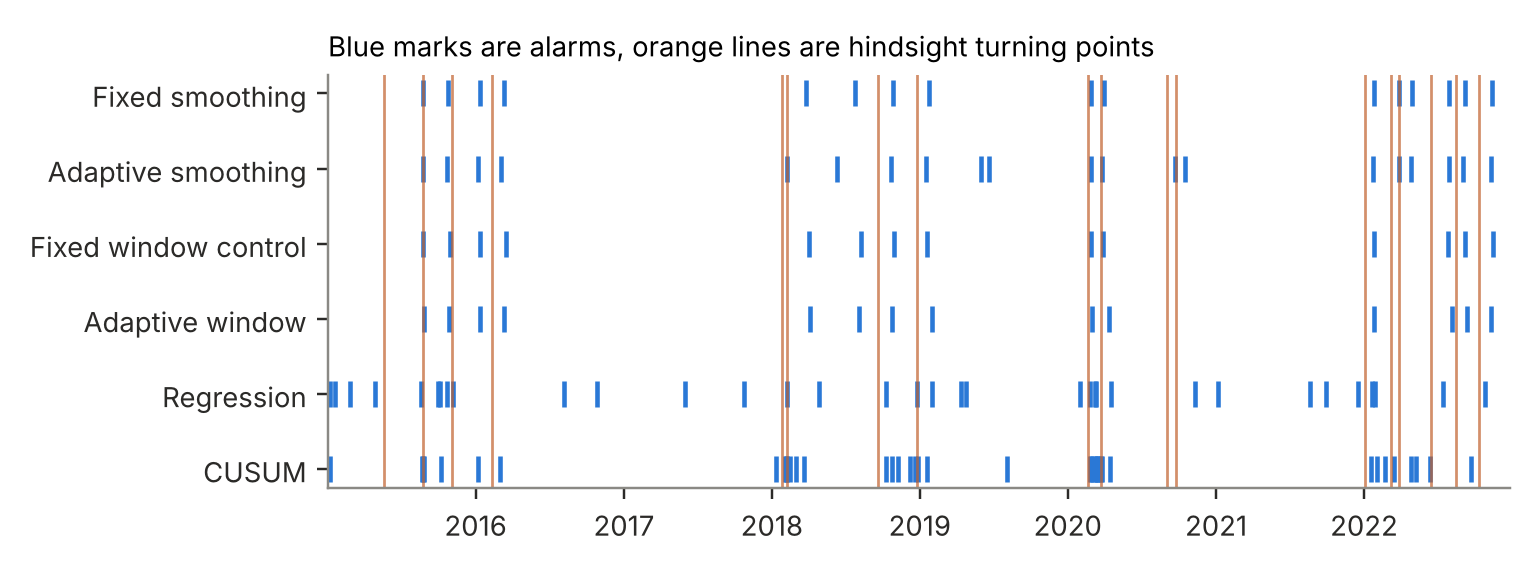
\includegraphics[width=\linewidth]{sp500_alarms.png}
\caption{Alarms on the test period, by method.}\label{fig:alarms}\end{figure}
Fixed smoothing scored highest at 0.765. Adaptive smoothing scored 0.737, catching one more turning point and reacting about two days sooner on average, but with four more alarms. The fixed and adaptive window methods tied at 0.688, with different alarm dates. All four trend methods beat random alarms ($p<0.001$). Regression and CUSUM did not clearly do so ($p=0.143$ and $0.149$). These results do not show either as useless, since neither targets the reversals in this answer key.

Tuned settings were $\alpha=0.3,\delta=0.07$ for fixed smoothing; $\alpha_{\min}=0.05,\alpha_{\max}=0.4,\delta=0.05$ for adaptive smoothing; $L=10,\delta=0.10$ for the fixed window; $L_{\min}=20,L_{\max}=40,c=2.5,\delta=0.07$ for the adaptive window; $L=120,k=4,d^*=3$ for regression; and $\kappa=0.25,h=5$ for CUSUM. Tuning-period results are in Table~\ref{tab:tune}. In that period the adaptive window (0.737) led the fixed window (0.667), but this advantage disappeared in testing, which illustrates why a separate test period is needed.
\begin{table}[ht]\centering\small\setlength{\tabcolsep}{4pt}
\caption{S\&P 500 tuning period, 2005--2014, with 18 turning points. These scores are in-sample.}\label{tab:tune}
\begin{tabular}{lcccccccc}\toprule
Method & Alarms & Hits & Prec. & Recall & $F_1$ & Delay & Random $F_1$ & $p$\\\midrule
\tabinput{tables/sp500_tune.tex}
\bottomrule\end{tabular}\end{table}

\section{Sensitivity}
Table~\ref{tab:sens} varies the answer-key size and time allowance after the settings are frozen. Adaptive smoothing beats fixed smoothing at 20 and 60 days under the 10\% key and throughout the 7\% key, but loses throughout the 15\% key. The ranking between them therefore depends on the scoring definition, which is what the paper's warning about threshold dependence would lead us to expect.
\begin{table}[ht]\centering\small\setlength{\tabcolsep}{5pt}
\caption{Test-period $F_1$ under other answer-key sizes $\Delta$ and allowances $H$.}\label{tab:sens}
\begin{tabular}{lccccccccc}\toprule
& \multicolumn{3}{c}{$\Delta=7\%$} & \multicolumn{3}{c}{$\Delta=10\%$} & \multicolumn{3}{c}{$\Delta=15\%$}\\
Method & 20 & 40 & 60 & 20 & 40 & 60 & 20 & 40 & 60\\\midrule
\tabinput{tables/sensitivity.tex}
\bottomrule\end{tabular}\end{table}

\section{Adaptive behaviour during the COVID-19 crash}
Figure~\ref{fig:smooth} shows that $\alpha_t$ rises during the sustained fall in early 2020 and the adaptive line follows it more closely than a slow fixed line. Figure~\ref{fig:window} shows the window length resetting and regrowing. The adaptive rules behave as intended, even though this did not yield a clear overall gain.
\begin{figure}[ht]\centering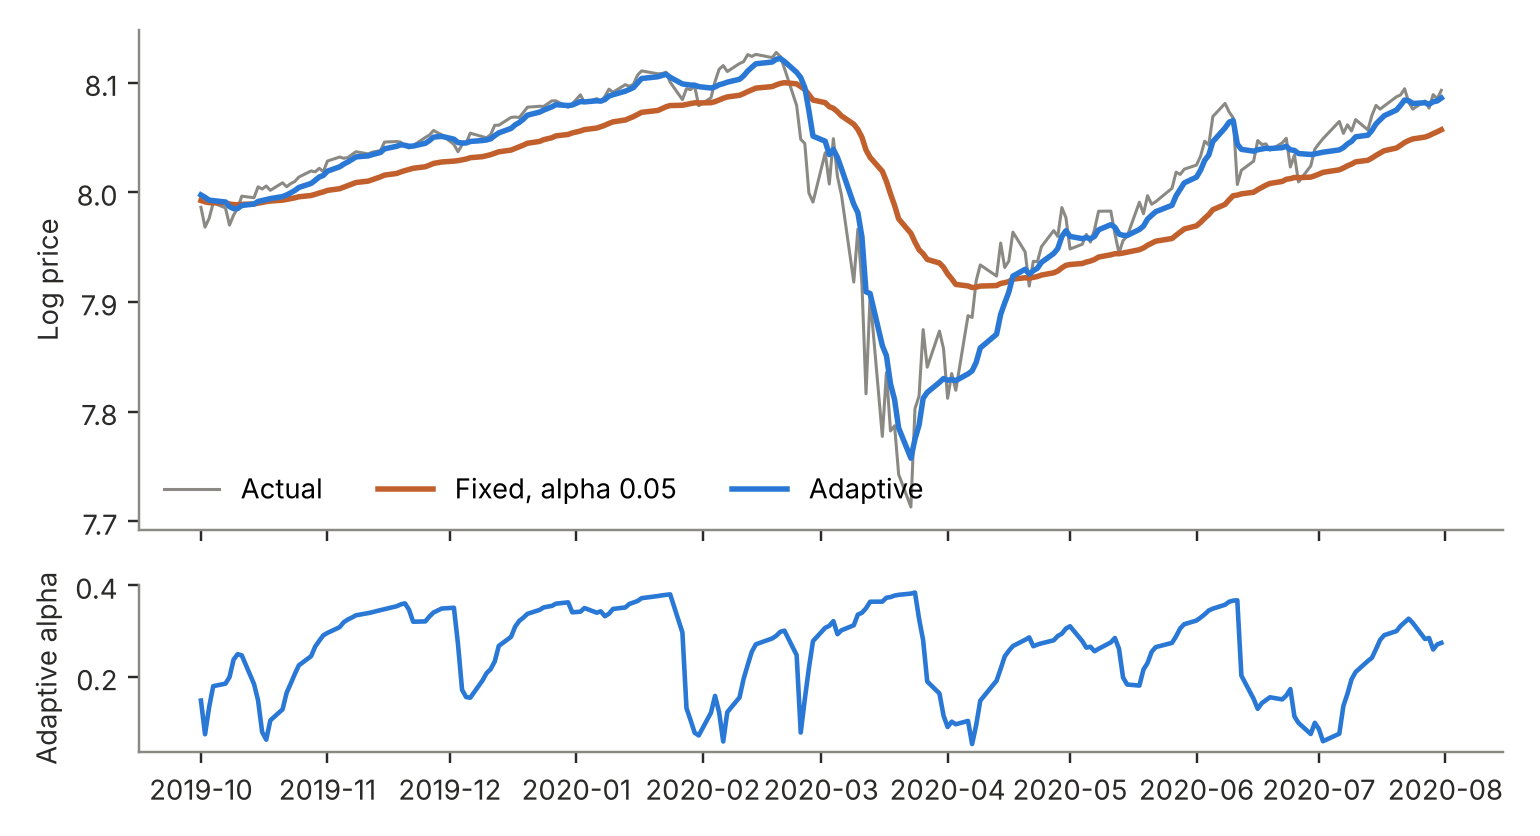
\includegraphics[width=\linewidth]{smoothing_comparison.png}
\caption{Fixed and adaptive smoothing around the 2020 crash, and the adaptive $\alpha_t$.}\label{fig:smooth}\end{figure}
\begin{figure}[ht]\centering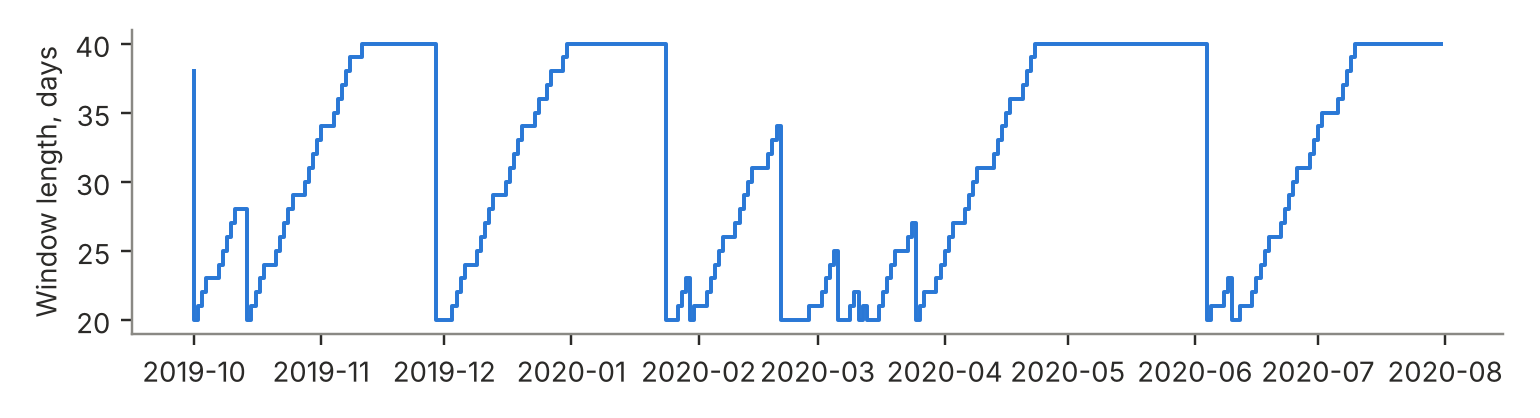
\includegraphics[width=\linewidth]{window_length.png}
\caption{Adaptive window length over the same dates.}\label{fig:window}\end{figure}

\section{Machine learning}
Table~\ref{tab:ml} compares the models with the rule on the same test period. 17.5\% of test days have target value 1, which is the average precision expected from uninformed guessing. Gradient boosting reached 0.440 and logistic regression 0.327, so the inputs carry information. Yet as alarm systems they scored $F_1=0.500$ and $0.444$, below the fixed smoothing rule. In a Case~B simulation, with 30 training runs, 10 runs for choosing the alarm level and 50 for testing, gradient boosting scored 0.499 and the rule 0.627. Both real-data models exceeded random alarms at $p=0.021$.
\begin{table}[ht]\centering\small
\caption{Machine learning and rule on the 2015--2022 test period. AP is average precision.}\label{tab:ml}
\begin{tabular}{lccccccc}\toprule
Model & Alarms & Hits & Prec. & Recall & $F_1$ & AP & $p$\\\midrule
\tabinput{tables/ml.tex}
\bottomrule\end{tabular}\end{table}

\chapter{Discussion}
\section{Why adaptation did not clearly win}
Proposition~\ref{prop:tradeoff} suggests one explanation. Adapting moves the estimator along the delay-noise curve; it does not remove the curve. In addition, $\delta$ is tuned for each method and already controls false alarms. A tuned $\alpha=0.3$ with $\delta=0.07$ leaves less room for an adaptive gain to matter. Adaptive methods also add settings, which increases the risk of fitting the tuning period, as the adaptive window's tuning lead suggests. These explanations are plausible rather than proven here, and could be tested by simulation.
\section{Relation to the paper}
The results agree with the paper on three points: thresholds and definitions strongly affect the outcome, no method is universally best, and detectors should match the task. They go further in measuring adaptivity against fixed controls, and find a small and inconsistent gain in this daily-index setting. They do not contradict the paper's minute-level currency examples, because the data and implementation differ.
\section{Limitations}
\begin{itemize}
\item \textbf{One history, few events.} The real test has 18 turning points, so small $F_1$ gaps cannot be resolved. We have not given a formal test of the difference between fixed and adaptive smoothing on real data.
\item \textbf{Answer-key alignment.} The turning-point key and the shared alarm rule have similar logic, which favours trend methods over CUSUM and regression. Real-data comparisons across these groups must be read with care.
\item \textbf{Asymmetric tuning.} Methods have different numbers of settings and grids. Tuning on real data was also done on one path with a small number of events.
\item \textbf{Related series.} The 20 companies belong to the index, creating a built-in link. They come from a recent list, introducing survivorship bias. A cleaner test would use the Nasdaq, Dow Jones and Russell 2000, as the repository's Yahoo option allows.
\item \textbf{Period.} The data end in December 2022, and the sample is daily. No conclusion is drawn about higher frequencies.
\item \textbf{No profit test.} Costs and trading performance were not studied, so no trading conclusion follows.
\item \textbf{Scope.} Bidirectional filtering, the five-point inflection rule and precedent matching from the paper are not implemented. The specific adaptive rules are our own choices, so results apply to them and not to all possible adaptive methods.
\end{itemize}

\chapter{Conclusion and Future Work}
We asked whether online adaptation improves change point detection over a tuned fixed setting. In this study, it did not do so reliably. Its effect ranged from negligible to mildly positive or mildly negative by method and noise type. On the S\&P~500 test years, a simple fixed smoother was at least as good as the alternatives, and machine learning models did not beat it. Results also confirmed that a detector must match the type of change sought. The practical lesson is to always test an adaptive or complex method against a tuned simple control, using data not used for tuning.

Future work includes: extending the data to 2025 and using index-level related series; testing other markets such as the Nifty~50; adding the paper's bidirectional filter and precedent matching; using walk-forward retuning; and applying the methods to climate, seismic or medical series.

\begin{thebibliography}{99}\small
\bibitem{musaev2024} A.~Musaev, D.~Grigoriev, M.~Kolosov. Adaptive algorithms for change point detection in financial time series. \emph{AIMS Mathematics}, 9(12):35238--35263, 2024. doi:10.3934/math.20241674.
\bibitem{sklearn} F.~Pedregosa et al. Scikit-learn: machine learning in Python. \emph{Journal of Machine Learning Research}, 12:2825--2830, 2011.
\bibitem{skfolio} skfolio contributors. skfolio: portfolio optimization built on scikit-learn. Python package, version 1.12.5, \url{https://github.com/skfolio/skfolio}.
\end{thebibliography}
\end{document}
